% Hanner-Hydra paper.
%
% Portable article-class source that arXiv compiles as is. For the journal submission
% (target: Data Mining and Knowledge Discovery), switch to Springer Nature's sn-jnl class
% (LaTeX template v3.1); see README.md. Keep the section files free of class-specific
% macros so that the switch only touches this file.
\documentclass[11pt]{article}

\usepackage[T1]{fontenc}
\usepackage{lmodern}
\usepackage[a4paper,margin=2.5cm]{geometry}
\usepackage{amsmath,amssymb,amsthm}
\usepackage{booktabs}
\usepackage{graphicx}
\usepackage{xcolor}
\usepackage[section]{placeins} % keep floats inside their section
\usepackage[numbers,sort&compress]{natbib}
\usepackage[hidelinks]{hyperref}

\newtheorem{theorem}{Theorem}
\newtheorem{proposition}[theorem]{Proposition}
\theoremstyle{definition}
\newtheorem{definition}[theorem]{Definition}

% Notation shared by all sections.
\newcommand{\R}{\mathbb{R}}
\newcommand{\linf}{\oplus_\infty}
\newcommand{\lone}{\oplus_1}
\newcommand{\hh}{Hanner-Hydra}

% Outline markers: visible in the draft, removed before submission.
\newcommand{\paperoutline}[1]{\par\noindent\textcolor{gray}{\textsf{[Outline] #1}}\par}
\newcommand{\todo}[1]{\textcolor{red}{\textsf{[TODO: #1]}}}

\title{Hanner-Hydra: Multiplication-Free Competing Kernels from Hanner Polytopes
  for Time Series Classification}
\author{J\"org Bahlmann\\\small Independent Researcher, L\"ubeck, Germany\\\small \href{mailto:joerg@bahlmann.ai}{joerg@bahlmann.ai}\\\small ORCID \href{https://orcid.org/0009-0009-6497-6823}{0009-0009-6497-6823}}
\date{Draft, \today}

\begin{document}
\maketitle

\begin{abstract}
Hydra classifies time series by letting random convolutional kernels compete in groups and
counting the winners. Finding the winner of a group of $k$ kernels of length $\ell$ costs
$k\ell$ multiplications per time step. We replace each group by the vertex set of a Hanner
polytope, a convex body built from segments by products and $\ell_1$ sums. Its vertices are
ternary, and its support function follows the tree of its construction, so the winner of a
group with up to $2^\ell$ vertices costs $\ell$ absolute values and $\ell-1$ additions or
comparisons, with no multiplication. We evaluated \hh{} in a pre-registered study on 112
UCR and 26 UEA datasets with 30 resamples each, against Hydra and two theory-matched
ternary controls, with a Bayesian non-inferiority rule (ROPE $\pm0.5$ accuracy points).
\hh{} is practically equivalent to Hydra in accuracy ($-0.06$ points, posterior
probability 0.988 of being not worse). Its single-core transform is $11.2\times$ faster
(95\% interval 10.2--12.0) and needs $23.8\times$ less memory. The result is equivalence,
not improvement: on the UEA datasets alone, \emph{not worse} is not shown. \hh{} is
equivalent to both controls, so the tree structure contributes speed, $3.8\times$ over a
dense ternary evaluation of the same groups, but not accuracy. The code, the
pre-registration and all per-case results are public.
\end{abstract}

\section{Introduction}
\label{sec:introduction}

Methods built on random convolutional kernels combine accuracy and speed better than most
other approaches to time series classification
\citep{dempster2020rocket,dempster2021minirocket,tan2022multirocket,middlehurst2024bakeoff}.
Hydra \citep{dempster2023hydra} organises such kernels into groups that compete at every
time step and counts how often each kernel wins, which links convolutional methods with
dictionary methods that count patterns. Together with MultiRocket features, Hydra is among
the most accurate methods on the UCR archive \citep{middlehurst2024bakeoff}.

The competition has a cost. To find the winner of a group of $k$ kernels of length $\ell$,
Hydra evaluates every kernel: $k\ell$ multiplications per group and time step. Work on edge
devices makes each kernel cheaper. NanoHydra \citep{cioflan2025nanohydra} uses binary
kernels and integer arithmetic on a microcontroller, but still evaluates every kernel of a
group, and in its own evaluation it is 1.5 points less accurate than Hydra on the UCR
archive (83.81\% against 85.31\%), although its numbers are the best of several runs per
dataset. This paper asks a different question: can the winner of a group be found without
evaluating its kernels one by one, without losing accuracy?

We answer it with groups that have a structure. Each group of \hh{} is the vertex set of a
Hanner polytope, a convex body built from segments by products and $\ell_1$ sums
\citep{hanner1956intersections,hansen1981structure}. In the canonical coordinates, every
vertex is a ternary vector in $\{-1,0,1\}^\ell$, and the polytope's support function follows
the tree of its construction. The winning vertex of a group with up to $2^\ell$ vertices
then costs $\ell$ absolute values and $\ell-1$ additions or comparisons, and no
multiplications. The winners are sign patterns on subsets of the taps, the codes of
hyperplane and cross-polytope hashing \citep{charikar2002simhash,andoni2015crosspolytope}.
Hanner polytopes also have an extremal property: they minimise the volume product among
unconditional bodies, and an unrefereed 2026 manuscript claims that they are the equality
cases of the symmetric Mahler conjecture in general \citep{openai2026mahler}. The method does
not depend on this property (Section~\ref{sec:background}).

A cheaper group is only useful if it does not cost accuracy, and a fast new kernel family
invites the question of which of its properties matter. We therefore tested a
non-inferiority hypothesis that we fixed in advance, with two controls matched to the
Hanner groups in size and sparsity: random ternary groups, and random ternary groups that
are centrally symmetric like every Hanner polytope.

Our contributions are:
\begin{itemize}
\item the Hanner kernel family, with a proof that the winner of a group follows its tree in
  $O(\ell)$ operations, including an exact rule for ties (Section~\ref{sec:method});
\item two theory-matched controls that separate the tree structure from ternary weights
  and from central symmetry (Section~\ref{sec:controls});
\item a pre-registered evaluation on 138 UCR and UEA datasets with 30 resamples each, a
  non-inferiority decision rule and a controlled single-core timing protocol
  (Section~\ref{sec:protocol});
\item a NumPy reference implementation, Numba kernels that reproduce it bit for bit,
  aeon-compatible estimators, and the full per-case results (Section~\ref{sec:reproducibility}).
\end{itemize}

The pre-registered hypothesis is accepted (Section~\ref{sec:results}). \hh{} is practically
equivalent to Hydra in accuracy, $-0.06$ points with a posterior probability of 0.988 of
being not worse, and to the matched controls. Its single-core transform is $11.2\times$
faster than Hydra's, and it needs $23.8\times$ less memory. The result is one of
equivalence, not improvement, and it has limits: on the UEA datasets alone, \emph{not
worse} is not shown, the gap to Hydra on balanced accuracy and macro-F1 is inconclusive,
and MultiRocket and HIVE-COTE~2.0 remain more accurate. The tree structure contributes
speed, not accuracy. Section~\ref{sec:background} reviews Hydra and Hanner polytopes,
Section~\ref{sec:related} discusses related work, and Section~\ref{sec:discussion} the
limitations.

\section{Background}
\label{sec:background}

\subsection{Hydra}
\label{sec:hydra}

Hydra \citep{dempster2023hydra} transforms a time series with random convolutional kernels
organised into competing groups. In the configuration we compare against, each group has
$k=8$ kernels of length 9 with Gaussian weights, and there are $g=64$ groups per dilation,
half applied to the series and half to its first difference. The dilations grow
exponentially, and the convolutions are padded so that the output has the length of the
input. In a multivariate series, each group works on the sum of a random subset of
channels.

At every time step, each group compares the responses of its $k$ kernels. Hydra records two
counts per kernel: a \emph{soft} count, which adds the response of the kernel with the
largest response, and a \emph{hard} count of how often the kernel has the smallest response
(the \emph{hard-min} count). The features of all groups go through a sparse scaler and a
ridge classifier. The size of the groups moves Hydra between ROCKET-like features
\citep{dempster2020rocket} and dictionary-like counts of patterns
\citep{dempster2023hydra}.

Geometrically, the kernels $w_1,\dots,w_k\in\R^\ell$ of a group are points, and the winner
for a patch $x$ is the point that maximises $\langle x,w_j\rangle$. It is the vertex of the
polytope $P=\operatorname{conv}\{w_1,\dots,w_k\}$ whose normal cone contains $x$: the group
divides $\R^\ell$ into cones and reports which cone each patch falls into, and the largest
response is the support function $h_P(x)=\max_j\langle x,w_j\rangle$. Finding the winner by
evaluating every kernel costs $k\ell$ multiplications per time step and group. \hh{} keeps
this pipeline and replaces $P$ by a polytope whose winner can be found without evaluating
its vertices one by one.

\subsection{Hanner polytopes}
\label{sec:hanner}

Hanner polytopes are the convex bodies built from the segment $[-1,1]$ by two operations,
the $\ell_\infty$ product $K_1\linf K_2=K_1\times K_2$ and the $\ell_1$ sum
$K_1\lone K_2=\operatorname{conv}((K_1\times\{0\})\cup(\{0\}\times K_2))$, together with
their linear images. They originate in Hanner's study of normed spaces in which every three
pairwise intersecting balls have a common point \citep{hanner1956intersections}; Hansen and
Lima showed that, in finite dimensions, these are exactly the spaces whose unit balls are
built in this way \citep{hansen1981structure}. The cube (products only) and the
cross-polytope (sums only) are the two extremes. Every Hanner polytope is described by a
rooted tree whose leaves are segments and whose internal nodes are products or sums. Trees
of this kind describe cographs, where they are called cotrees
\citep{corneil1981cographs}; we use the term for our labelled trees on the taps of a kernel
(Section~\ref{sec:groups}).

Hanner polytopes are extremal for several problems about centrally symmetric convex bodies.
Every Hanner polytope of dimension $d$ has exactly $3^d$ non-empty faces, the smallest
number that Kalai's $3^d$ conjecture allows for a centrally symmetric $d$-polytope; the
conjecture is proven for $d\le4$ \citep{sanyal2009kalai}, and among the Hansen polytopes
of graphs, the Hanner polytopes are exactly those of threshold graphs
\citep{freij2013hansen}.

The best-known extremal property concerns the volume product. For an origin-symmetric
convex body $K\subset\R^n$ with polar body $K^\circ$, Mahler conjectured that
$|K|\,|K^\circ|\ge 4^n/n!$ \citep{mahler1939uebertragung}. The cube and the cross-polytope
attain this value, and so does every Hanner polytope. The inequality was proven for
unconditional bodies \citep{saintraymond1981}, with the Hanner polytopes as the equality
cases in that class \citep{meyer1986caracterisation}, for zonoids
\citep{reisner1986zonoids}, and in dimension three
\citep{iriyeh2020mahler,fradelizi2022mahler}. The cube is a strict local minimiser of the
volume product \citep{nazarov2010mahler}, and so is every Hanner polytope
\citep{kim2014hanner}. In 2026, OpenAI released a manuscript that claims the full symmetric
conjecture, with equality exactly for the linear images of Hanner polytopes
\citep[Theorem~1.1]{openai2026mahler}. The manuscript is not peer reviewed; its repository
lists Lean formalisations of both the inequality and the equality characterisation, with
their review status recorded as unchecked.

Our method uses none of this extremality, and none of it implies that Hanner polytopes make
good kernel groups. The volume product is invariant under linear maps, so its minimisers
single out no coordinates, and it says nothing about how evenly the normal cones of a
polytope divide $\R^\ell$, which is what matters for a group of competing kernels. \hh{}
relies only on three properties that every Hanner polytope has in its canonical coordinates,
whatever the status of the Mahler conjecture: its vertices are ternary, it is centrally
symmetric, and its support function and winning vertex follow its tree
(Section~\ref{sec:method}). The extremal results are why we looked at this family; the
experiments, not the theory, decide whether it makes good kernel groups.

\section{Method}
\label{sec:method}

\hh{} keeps Hydra's pipeline (dilated convolutions on the series and its first difference,
competing groups, counts of winners, sparse scaling and a ridge classifier) and changes
only the groups. Each group is the vertex set of a Hanner polytope, given by a labelled
cotree on the kernel's taps. This section defines the groups
(Section~\ref{sec:groups}), shows that the winner of a group follows the cotree
(Section~\ref{sec:recursion}), interprets the resulting features
(Section~\ref{sec:interpretation}), and describes the sampler, the transform, the
operation count, the controls and the implementation
(Sections~\ref{sec:sampling}--\ref{sec:implementation}).

\subsection{Hanner groups}
\label{sec:groups}

A kernel has $\ell$ taps, and a patch is a vector $x\in\R^\ell$ of $\ell$ dilated samples of
the input. A \emph{labelled cotree} $T$ on the taps is a full binary tree whose leaves are
the taps $1,\dots,\ell$, each exactly once, and whose internal nodes are labelled $\lone$
(an $\ell_1$ sum) or $\linf$ (an $\ell_\infty$ product). Every subtree $S$ covers a set
$\tau(S)$ of taps, and the two children of a node cover disjoint sets.

\begin{definition}[Hanner group]
\label{def:group}
The \emph{group} of a subtree $S$ is the ordered list $V(S)$ of vectors in $\R^\ell$
defined by
\begin{itemize}
\item a leaf on tap $i$: $V(S)=(-e_i,\,e_i)$;
\item $S=S_1\lone S_2$: the list $V(S_1)$ followed by $V(S_2)$;
\item $S=S_1\linf S_2$: the vectors $v_a+u_b$ for $v_a\in V(S_1)$, $u_b\in V(S_2)$,
  ordered by the index $a\,n_2+b$, where $n_2=|V(S_2)|$ and indices start at 0.
\end{itemize}
The group of the cotree is $V=V(T)$, and its size is $|V|$.
\end{definition}

The convex hull of $V$ is the Hanner polytope of $T$: a leaf gives the segment
$[-e_i,e_i]$, a $\linf$ node gives the Cartesian product $K_1\times K_2$ of the
children's polytopes (they live in complementary coordinate subspaces), and a $\lone$ node
gives $\operatorname{conv}(K_1\cup K_2)$. These are the two operations that define Hanner
polytopes \citep{hanner1956intersections,hansen1981structure}.

\begin{proposition}[Structure of a group]
\label{prop:structure}
For every labelled cotree $T$ on $\ell$ taps:
\begin{enumerate}
\item the vectors in $V$ are distinct, and they are exactly the vertices of
  $\operatorname{conv}V$;
\item every vector has entries in $\{-1,0,1\}$, and its support is a union of whole
  leaves;
\item $V=-V$: the map $\alpha$ defined by swapping the two vertices of each leaf, acting
  on each part of a $\lone$ node and on both factors of a $\linf$ node, is an involution
  with $V_{\alpha(j)}=-V_j$;
\item $2\ell\le|V|\le 2^\ell$; the cross-polytope (all nodes $\lone$) attains the lower
  bound and the cube (all nodes $\linf$) the upper one.
\end{enumerate}
\end{proposition}

\begin{proof}
All four statements follow by induction over the tree. (1)~The vertices of a product of
polytopes are the pairs of vertices. For two polytopes in complementary subspaces that each
contain the origin in their relative interior, the vertices of the convex hull of their union
are the vertices of the two polytopes. Distinctness follows because the parts of a $\lone$
node have disjoint supports and the parts of a $\linf$ node are recovered by restricting to
$\tau(S_1)$ and $\tau(S_2)$. (2)~Each tap belongs to one leaf, and a $\linf$ node adds vectors
with disjoint supports. (3)~Negation commutes with both operations. (4)~A subtree on $t$
taps has between $2t$ and $2^t$ vertices: a leaf has 2; a $\lone$ node has $n_1+n_2$ and a
$\linf$ node $n_1n_2$ vertices, and $n_1+n_2\le n_1n_2$ whenever $n_1,n_2\ge2$. The bounds
are not characterisations: a product of two leaves has $4=2+2$ vertices, so, for example,
$(x_1\linf x_2)\lone x_3$ also has $2\ell=6$ vertices.
\end{proof}

\subsection{Support-function recursion}
\label{sec:recursion}

Hydra's group responds to a patch $x$ with the winning kernel
$\operatorname{arg\,max}_j\langle x,w_j\rangle$ and its response. For a Hanner group, the
response of the winner is the support function $h(x)=\max_{v\in V}\langle x,v\rangle$ of
the polytope, and it follows the cotree.

\begin{proposition}[Winner recursion]
\label{prop:recursion}
Compute, bottom-up over the cotree, a value $h(S)$ and an index $w(S)$ for every subtree:
\begin{itemize}
\item leaf on tap $i$: $h=|x_i|$; $w=1$ (the vertex $e_i$) if $x_i>0$, and $w=0$ (the
  vertex $-e_i$) otherwise;
\item $S=S_1\linf S_2$: $h=h(S_1)+h(S_2)$ and $w=w(S_1)\,n_2+w(S_2)$;
\item $S=S_1\lone S_2$: if $h(S_1)\ge h(S_2)$, then $h=h(S_1)$ and $w=w(S_1)$; otherwise
  $h=h(S_2)$ and $w=n_1+w(S_2)$, with $n_1=|V(S_1)|$.
\end{itemize}
At the root, $h(T)=\max_{v\in V}\langle x,v\rangle$, and $w(T)$ is the lowest index in $V$
at which this maximum is attained. The recursion uses $\ell$ absolute values and $\ell-1$
additions or comparisons of real numbers, and no multiplications; each leaf's sign test
$x_i>0$ yields both $|x_i|$ (by a select) and the leaf's winner.
\end{proposition}

\begin{proof}
By induction, with the claim that $h(S)=\max_{v\in V(S)}\langle x,v\rangle$ and that $w(S)$
is the lowest maximising index in $V(S)$.
\emph{Leaf.} The responses are $-x_i$ (index 0) and $x_i$ (index 1). If $x_i>0$, only
index~1 attains $|x_i|$; if $x_i<0$, only index~0; if $x_i=0$, both do and the lowest is~0.
\emph{Product.} Since $v_a$ and $u_b$ have disjoint supports,
$\langle x,v_a+u_b\rangle=\langle x,v_a\rangle+\langle x,u_b\rangle$, so the maximum is
$h(S_1)+h(S_2)$ and the set of maximisers is the product of the children's maximiser sets.
Because $0\le b<n_2$, the index $a\,n_2+b$ is lexicographic in $(a,b)$, so its minimum
over a product set is attained at the two smallest indices.
\emph{Sum.} $V(S)$ is the union of the two lists, with the first list at indices below
$n_1$, so the maximum is $\max(h(S_1),h(S_2))$. If $h(S_1)\ge h(S_2)$, the first list
contains a maximiser, and every index in it is lower than every index in the second.
Otherwise every maximiser is in the second list, at offset $n_1$.
\emph{Count.} A binary tree with $\ell$ leaves has $\ell-1$ internal nodes, each costing one
addition or one comparison. The index updates are integer arithmetic on the winners and do
not involve the data.
\end{proof}

The index $w(T)$ is the first maximiser in list order, which is what a brute-force argmax
over $V$ returns, so the recursion and a brute-force evaluation give the same winner and
the same counts, including ties. This
statement is about exact arithmetic. In floating point, the recursion adds the responses in
the order of the tree, while a dot product adds them in tap order. Our reference
implementation and the fast kernels both use the recursion's order and agree bit for bit
(Section~\ref{sec:implementation}).

\begin{proposition}[Minimum and hard-min counts]
\label{prop:hardmin}
For a Hanner group, $\min_{v\in V}\langle x,v\rangle=-h(x)$, attained at $\alpha(w)$. If the
minimiser is taken to be $\alpha(w)$, the hard-min count of every vertex $v$ equals the
hard-max count of $-v$, so the hard-min features are a fixed permutation of the hard-max
features. The same holds for every centrally symmetric group.
\end{proposition}

This follows from $V=-V$ (Proposition~\ref{prop:structure}). The tie rule matters: Hydra
takes the \emph{first} minimiser in list order, which differs from $\alpha(w)$ whenever the
minimum is attained more than once. Ties are not rare: a patch with a zero tap, as at the
zero-padded ends of a series, ties at that leaf. With Hydra's rule the hard-min counts are
therefore a permutation of the hard-max counts only up to tied patches. Our implementation
uses $\alpha(w)$. A per-feature scaler and a linear classifier are invariant to a fixed
permutation of the features, so these hard-min counts carry no information beyond the
hard-max counts, and \hh{} counts soft maxima and hard maxima (Section~\ref{sec:transform}).
The ablation with hard-min counts (Section~\ref{sec:results}) uses the same $\alpha(w)$
rule; its identical predictions confirm the permutation argument in the implementation,
but they are not an independent test of Hydra's first-minimiser rule.

\subsection{What the features compute}
\label{sec:interpretation}

The two extreme cotrees give two familiar codes. For the cube ($|V|=2^\ell$, all
$\linf$), the winner is the sign pattern of the patch,
$(\operatorname{sign}x_1,\dots,\operatorname{sign}x_\ell)$ with $0$ mapped to $-1$, and $h$
is $\|x\|_1$. This is the code of hyperplane hashing \citep{charikar2002simhash}, here with
the coordinate axes as hyperplanes. For the cross-polytope ($|V|=2\ell$, all $\lone$), the
winner is the coordinate of largest magnitude with its sign, and $h=\|x\|_\infty$. This is
the code of cross-polytope hashing \citep{andoni2015crosspolytope}, without its random
rotation. In a mixed cotree, a $\linf$ node concatenates the winners of its children and a
$\lone$ node keeps the winner of the child with the larger response. The winner is
therefore a sign pattern on a subset of the taps, and the $\lone$ nodes choose the subset
by where the patch responds most strongly. In \hh{} the randomness that hashing gets from
random projections comes from the sampled cotree, the dilation and the channel subset.

The features are therefore close to counts of binary symbolic words, as in dictionary
methods \citep{lin2007sax,schaefer2023weasel2}, and to sign patterns of neighbouring
samples \citep{kaya2014lbp}. They differ from ordinal patterns \citep{bandt2002permutation},
which record the rank order of the samples rather than their signs. The soft-max count
weights each word by the response $h$, which, for a cube on centred taps, is the patch's
$\ell_1$ deviation from its mean.

\subsection{Cotree sampling}
\label{sec:sampling}

Groups are drawn at random under a vertex budget $V_{\max}$. The sampler starts from the
$\ell$ leaves in random order and merges two randomly chosen subtrees until one tree
remains. A merge of subtrees with $n_a$ and $n_b$ vertices is a $\linf$ product with
probability $p_{\text{product}}$ if
\[
  R + n_a n_b \le V_{\max},
\]
where $R$ is the total vertex count of the other subtrees; otherwise it is a $\lone$ sum.
Merging all remaining subtrees by sums would give $R+n_an_b$ vertices, the smallest
possible final count, so the condition keeps the final group within $V_{\max}$ and no draw
is ever rejected. Every tap appears in every group, so $2\ell\le|V|\le V_{\max}$. With the
frozen setting ($\ell=9$, $V_{\max}=32$, $p_{\text{product}}=0.5$), groups have 18 to 32
vertices, 24.4 on average (Table~\ref{tab:operations}). The sampler can also restrict
merges to adjacent blocks of taps; this option is off in all reported runs.

\subsection{The transform}
\label{sec:transform}

The transform follows Hydra \citep{dempster2023hydra} in everything but the groups.
\begin{itemize}
\item \emph{Dilations and inputs.} The dilations are $2^0,2^1,\dots,
  2^{\lfloor\log_2((T-1)/(\ell-1))\rfloor}$ for series of length $T$, with zero padding
  that keeps the output length. Each dilation is applied to the series and to its first
  difference.
\item \emph{Groups per block.} For each pair of dilation and input (a block), groups are
  drawn until their vertices, the \emph{atoms}, reach a budget of 256, the number of
  kernels Hydra uses per block ($k=8$ kernels in 32 groups). A block has 10.9 groups on
  average.
\item \emph{Channels.} For a series with $C>1$ channels, each group draws
  $\operatorname{clip}(\lfloor C/2\rfloor,2,8)$ channels at random (with replacement), the
  subset size used by Hydra, and works on their sum.
\item \emph{Centring.} In each block, every second group sees mean-centred patches
  $x-\bar{x}\mathbf{1}$, and the others see raw patches. The centred groups respond to the
  shape of a patch regardless of its level; the raw groups also see the level relative to
  zero (ablation in Section~\ref{sec:results}).
\item \emph{Features.} For every vertex $v$ of every group, the transform records the
  number of time steps at which $v$ wins (hard-max count) and the sum of the winning
  responses $h$ at those steps (soft-max count). A block contributes two features per
  atom.
\item \emph{Classifier.} The features go through Hydra's sparse scaler, which takes square
  roots, standardises each feature and sets the entries that were zero back to zero. A
  ridge classifier follows, with its regularisation strength chosen by leave-one-out
  cross-validation among 10 values from $10^{-3}$ to $10^{3}$.
\end{itemize}

\subsection{Operation count}
\label{sec:operations}

\begin{table}[t]
\centering\small
% Generated by experiments/paper_tables.py; do not edit by hand.
\begin{tabular}{lrrrrr}
\toprule
 & Vertices & Operations & Groups & Operations & Multipli- \\
 & per group & per group & per block & per block & cations \\
\midrule
Hydra (Gaussian) & 8 & 150 & 32 & 4,800 & 2,304 \\
Matched control, as timed (dense) & 24.4 & 438.8 & 10.9 & 4,804 & 2,408 \\
Matched control, sparse (not timed) & 24.4 & 54.4 & 10.9 & 596 & 0 \\
Hanner-Hydra (recursion) & 24.4 & 17 & 10.9 & 186 & 0 \\
\midrule
\multicolumn{6}{l}{Ratios per block: Hydra / Hanner 25.8$\times$, dense control / Hanner 25.8$\times$, sparse control / Hanner 3.2$\times$} \\
\multicolumn{6}{l}{(2,000 sampled blocks, seed 0)} \\
\bottomrule
\end{tabular}

\caption{Arithmetic per time step of one block (one dilation and input, 256 atoms), under
the frozen sampler. Operations are additions, subtractions, comparisons and, for Hydra,
multiplications; \hh{} also takes $\ell=9$ absolute values per group, included in its
count. The matched control has the same vertex sparsity as \hh{}. As timed, it evaluates
every vertex as a dense dot product over all $\ell$ taps, multiplying by $-1$, $0$ or $1$;
the sparse row counts an evaluation over the non-zeros only, which we did not implement.
Hydra finds both the maximum and the minimum of each group. Patch extraction, channel
sums, centring and counting are shared by all arms and not counted.}
\label{tab:operations}
\end{table}

Table~\ref{tab:operations} counts the arithmetic that finding the winners needs: the
intrinsic cost of a group, not a model of the measured times. A Hydra group of 8 Gaussian
kernels of length 9 costs 72 multiplications, 64 additions and 14 comparisons for 8 atoms.
A Hanner group costs 17 operations for 24 atoms on average, with no multiplication. A
ternary group with the same vertices costs 439 operations when every vertex is evaluated
densely, as in our control kernel, and 54 when only the non-zeros are visited. Per block,
Hydra and the dense control both need about $26\times$ the operations of \hh{}, and a
sparse control would need $3.2\times$.

The measured transform-time ratios do not follow these counts: Hydra / \hh{} is
$11.2\times$, \texttt{control\_sym} / \hh{} is $3.8\times$, and Hydra / \texttt{control\_sym}
is $3.0\times$, although Hydra and the dense control have nearly the same count
(Section~\ref{sec:results}). The shared costs in the caption (patch extraction, channel
sums and counting, which touch memory) take a large share of the time, and Hydra runs its
convolutions in PyTorch, in aeon's implementation. Two consequences for the comparison with
the controls: the $3.8\times$ compares the recursion with a dense ternary evaluation of the
same groups, so it is an upper bound on what the cotree adds over the best ternary
implementation; and the counts alone do not say how much of it a sparse control kernel would
recover. We did not time one.

\emph{What ``multiplication-free'' covers.} It covers the group evaluation: the winner and
its response need only absolute values, additions and comparisons. The first difference is
a subtraction, and soft-max counts add the winning responses. Centring is the one place
where our implementation divides: it subtracts the patch mean $\bar{x}=s/\ell$, with
$s=\sum_i x_i$, once per patch, not once per group or vertex. A multiplication-free form
exists: evaluate the group on $\ell x_i-s$ instead, where $9x_i=8x_i+x_i$ is a shift and an
addition for $\ell=9$. Since $\langle\ell x-s\mathbf{1},v\rangle=\ell\,\langle
x-\bar{x}\mathbf{1},v\rangle$, the winners and hard-max counts are unchanged in exact
arithmetic, and the soft-max counts of the centred groups are scaled by $\ell$, which the
per-feature scaler removes. The sparse scaler and the ridge classifier do multiply, as in
Hydra and MiniRocket. The kernels we timed use floating point and the division; all
timings are for that implementation, not for the scaled form.

\subsection{Theory-matched controls}
\label{sec:controls}

Two controls separate the cotree structure from the other properties of a Hanner group.
For every Hanner group, a control draws a random group of ternary vectors with the same
size and the same number of non-zeros per vertex: the positions and signs of the non-zeros
are uniform, and duplicate vectors are redrawn. \texttt{control} draws the vectors
independently. \texttt{control\_sym} draws them in antipodal pairs $(u,-u)$ placed at the
pair positions of the Hanner group, so it is centrally symmetric and has the same antipode
map $\alpha$. Both controls are evaluated by ternary dot products, $|V|$ per patch, each over all $\ell$
taps (Section~\ref{sec:operations}), and
pass through the same transform, scaler and classifier. A difference between \hh{} and
\texttt{control\_sym} can therefore come only from the cotree structure, and a difference
between the two controls only from central symmetry. The pre-registration names
\texttt{control\_sym} as the primary control (Section~\ref{sec:protocol}).

\subsection{Implementation}
\label{sec:implementation}

The reference implementation is written in NumPy. It fixes the order of every
floating-point sum, so that a second implementation can reproduce it exactly. The timed
implementation consists of single-threaded Numba kernels, one for Hanner groups (the
recursion of Proposition~\ref{prop:recursion}) and one for the ternary controls. The tests
check that both kernels reproduce the reference bit for bit, and that the recursion agrees
with brute force over the vertex list, including ties. The method is also available as
aeon estimators \citep{middlehurst2024aeon}, a transformer and a classifier that wrap the
reference and reproduce it exactly. Section~\ref{sec:reproducibility} lists the code and
data.

\section{Pre-registered protocol}
\label{sec:protocol}

We fixed the hypothesis, the configuration, the datasets, the analysis and the decision rule
before the main runs, and froze them on 4 November 2026 as a tagged commit of our
development repository. The pre-registration is a document in our own repository, not an
entry in a public registry, and the development history is not public, so its date is
not independently verifiable; the public copy records the SHA-256 of the frozen document. Pre-registration is still rare in machine
learning \citep{prereg2020neurips}. We use it because a non-inferiority claim depends on
choices (margin, metric, datasets, timing procedure) that are easy to adjust after seeing
the results. Section~\ref{sec:reproducibility} gives the document and the code. This section
summarises the protocol; the document itself takes precedence.

\paragraph{Hypothesis.} H1 states that \hh{} is not worse than Hydra and not worse than the
symmetric control in accuracy, and that its single-core transform is at least four times
faster than Hydra's. H0 is retained if any of the three conditions fails.

\paragraph{Arms.} \hh{}, \texttt{control\_sym} and \texttt{control} use the frozen
configuration of Section~\ref{sec:method} ($\ell=9$, $V_{\max}=32$,
$p_{\text{product}}=0.5$, 256 atoms per block, mixed centring, at most 8 channels per
group, soft-max and hard-max counts). Hydra is aeon's \texttt{HydraClassifier} with 8
kernels in 64 groups and its other defaults \citep{dempster2023hydra,middlehurst2024aeon}.
Before the freeze, this baseline reproduced aeon's published Hydra accuracies on the
default UCR splits (mean difference $+0.42$ points, within the pre-registered gate
of $\pm0.5$ points). Every arm is seeded with the resample
id.

\paragraph{Datasets and resamples.} We use the 112 UCR datasets of the Hydra evaluation and
the 26 equal-length UEA datasets \citep{dau2019ucr,bagnall2018uea}, 138 in all; the four
UEA datasets with series of unequal length are excluded, not padded. Each dataset has 30
resamples: resample 0 is the default train/test split, and resample $i>0$ pools the two and
redraws a stratified split with the original class counts, as in the bake-offs
\citep{ruiz2021multivariate,middlehurst2024bakeoff}. All arms see identical splits. A
dataset enters the analysis only if every arm completes all 30 resamples, and settings are
never changed for individual datasets.

\paragraph{Datasets that informed the design.} Development, diagnosis and pilot runs before
the freeze used 45 of the 138 datasets (28 UCR, 17 UEA). The pre-registration lists them,
and we report the other 93 (84 UCR, 9 UEA) separately as \emph{fresh} datasets.

\paragraph{Accuracy analysis.} The score of an arm on a dataset is its mean test accuracy
over the 30 resamples, in percentage points, and $\Delta$ is \hh{} minus the comparator. A
single Bayesian signed-rank test \citep{benavoli2017bayesian} over the 138 datasets, with a
region of practical equivalence (ROPE) of $\pm0.5$ points, gives the posterior
probabilities that \hh{} is practically worse, equivalent or better. \hh{} is \emph{not
worse} than a comparator if $P(\text{rope})+P(\text{better})\ge0.95$.

\paragraph{Timing analysis.} Times are measured on one machine (Apple M4, 32\,GB, on mains
power, Low Power Mode off, no other workload), with one thread per process. The timed
region is \texttt{transform} of the test set of the default split after \texttt{fit} on
the training set. For Hydra it includes aeon's conversion to and from PyTorch tensors; for
\hh{} it uses the Numba kernels. Neither the scaler nor the classifier is timed. Per
dataset, each arm gets one untimed warm-up and then seven timed calls, interleaved across
arms in a rotating order, and its time is the median of the seven. Three passes run in
separate processes, each with its own seeded dataset order, and the time of an arm on a
dataset is the median of its three pass medians. The endpoint is the median over the 138
datasets of the per-dataset ratio of Hydra's time to \hh{}'s.

\paragraph{Decision rule.} H1 is accepted if and only if \hh{} is not worse than Hydra, not
worse than \texttt{control\_sym}, and the median time ratio is at least 4.

\paragraph{Secondary analyses.} The pre-registration also names analyses that are reported
but do not decide: the subsets (UCR, UEA, fresh); the comparison with \texttt{control};
two-sided Wilcoxon signed-rank tests with Holm's correction and critical-difference
diagrams \citep{demsar2006statistical}; balanced accuracy and macro-F1; aeon's published
results for WEASEL~2.0, MiniRocket, MultiRocket and HIVE-COTE~2.0 on the UCR datasets;
peak transform memory; fit times; and exploratory ablations. Cache-miss rates were planned
as well, with the fallback of dropping them if the processor's counters could not be read
reliably; they could not, so they are not reported.

\paragraph{Deviation.} One change was made after the freeze. The frozen analysis code took
the order of the resamples from a set, whose iteration order depends on the process, so the
dataset means could differ in the last bit between runs and change the win/tie/loss counts,
which count exact ties, by one or two datasets. The fix sorts the resamples. It changes no
mean, no probability at the reported precision, and no decision.

\paragraph{Execution.} All arms completed all 30 resamples on all 138 datasets, so no
dataset was excluded (16,560 prediction files). The accuracy runs were interrupted twice
when the machine ran out of memory and stopped once by a memory watchdog; each time they
were resumed with identical seeds and code, and the interrupted resamples were rerun. All three
timing passes completed on every dataset. The first run of one pass took place while the
machine was in use, which breaks the idle condition, so it was repeated as the protocol
requires; the endpoint is the same with either run ($11.23\times$).

\section{Results}
\label{sec:results}

All three pre-registered conditions hold, so H1 is accepted. \hh{} is not worse than Hydra
and not worse than the symmetric control in accuracy, and its transform is $11.2\times$
faster than Hydra's. The accuracy result is one of equivalence, not superiority, and it is
not shown on the UEA datasets alone. All tables in this section are generated from the
stored results (Section~\ref{sec:reproducibility}).

\subsection{Primary endpoint}

\begin{table}[t]
\centering\small
% Generated by experiments/paper_tables.py; do not edit by hand.
\begin{tabular}{lrrlcc}
\toprule
Comparison & Means (\%) & $\Delta$ & W/T/L & $P$(left / rope / right) & $P$(not worse) \\
\midrule
vs Hydra & 84.37 vs 84.43 & $-0.06$ & 47/5/86 & 0.012 / 0.988 / 0.000 & \textbf{0.988} \\
vs \texttt{control\_sym} & 84.37 vs 84.33 & $+0.04$ & 64/7/67 & 0.000 / 1.000 / 0.000 & \textbf{1.000} \\
vs \texttt{control} & 84.37 vs 84.26 & $+0.11$ & 72/5/61 & 0.000 / 1.000 / 0.000 & \textbf{1.000} \\
\bottomrule
\end{tabular}

\caption{Primary endpoint: \hh{} against each arm over 138 datasets (dataset means over 30
resamples, percentage points). $\Delta$ is \hh{} minus the comparator; W/T/L counts
datasets. Bayesian signed-rank test with ROPE $\pm0.5$; bold: $P(\text{not worse})\ge
0.95$.}
\label{tab:primary}
\end{table}

\begin{table}[t]
\centering\small
% Generated by experiments/paper_tables.py; do not edit by hand.
\begin{tabular}{lr}
\toprule
Quantity (median over datasets) & Value \\
\midrule
Hydra / Hanner-Hydra transform time & 11.23$\times$ \\
\texttt{control\_sym} / Hanner-Hydra & 3.79$\times$ \\
Hydra / \texttt{control\_sym} & 2.99$\times$ \\
Smallest Hydra / Hanner-Hydra ratio & 4.06$\times$ \\
Datasets & 138 \\
\bottomrule
\end{tabular}

\caption{Single-core transform time (Apple M4, one thread). Per dataset, the median of
three pass medians; the table gives the median over datasets of the per-dataset ratios.}
\label{tab:timing}
\end{table}

Table~\ref{tab:primary} gives the accuracy comparisons. Against Hydra, the mean accuracy is
84.37\% against 84.43\% ($\Delta=-0.06$ points), and the posterior probability that \hh{}
is not worse is 0.988, all of it from the ROPE. Against \texttt{control\_sym} and
\texttt{control}, the posterior lies entirely in the ROPE. The differences per dataset are
small but not uniform. \hh{} loses more datasets to Hydra than it wins (47/5/86), with a
median difference of $-0.10$ points. On 18 of the 138 datasets the difference exceeds 2
points in either direction, from $-5.43$ (FreezerSmallTrain) to $+6.79$
(SemgHandMovementCh2).

Table~\ref{tab:timing} gives the timing endpoint. The median ratio of Hydra's transform time
to \hh{}'s is $11.23\times$, with a bootstrap 95\% interval of 10.23--12.01; the medians
of the three passes are $11.17\times$, $11.24\times$ and $11.24\times$. Every dataset is
above the pre-registered threshold of $4\times$. The ratio is $11.76\times$ on the UCR
datasets and $9.38\times$ on the UEA datasets. Summed over all datasets, one transform of
every test set takes 29.0 minutes with Hydra and 2.2 minutes with \hh{}.

\subsection{Where the speed comes from}

The controls split the speed-up into two parts. \texttt{control\_sym} runs in a Numba
kernel like \hh{}'s, but evaluates every vertex of its groups as a dense ternary dot
product instead of following a cotree. It is $2.99\times$ faster than Hydra and $3.79\times$
slower than \hh{}. The $3.79\times$ is the gain of the recursion over a dense ternary
evaluation of groups of the same size and sparsity. A ternary kernel that visits only the
non-zeros would need fewer operations (Table~\ref{tab:operations}), and we did not time
one, so $3.79\times$ is an upper bound on what the cotree adds over the best ternary
implementation (Section~\ref{sec:operations}). The operation counts are not a model of
these times: Hydra and the dense control have nearly the same count, but Hydra is
$2.99\times$ slower.

The ratio to Hydra is lowest on the two datasets with the most channels, DuckDuckGeese
($C=1{,}345$, $4.06\times$) and PEMS-SF ($C=963$, $4.83\times$), and on the dataset with
the longest series, StandWalkJump ($T=2{,}500$, $5.86\times$). It is highest for StarLightCurves
($23.15\times$). Seventeen datasets are below $8\times$.

\begin{table}[t]
\centering\small
% Generated by experiments/paper_tables.py; do not edit by hand.
\begin{tabular}{lr}
\toprule
Arm & Median extra peak memory (MB) \\
\midrule
Hanner-Hydra & 19 \\
\texttt{control} & 17 \\
\texttt{control\_sym} & 17 \\
Hydra & 450 \\
\midrule
Hydra / Hanner-Hydra (median of per-dataset ratios) & 23.8$\times$ \\
\bottomrule
\end{tabular}

\caption{Extra peak memory of the transform: the rise in peak resident set size during
\texttt{transform} of the test set, after \texttt{fit} and a warm-up, each measured in a
fresh process. It includes the output array.}
\label{tab:memory}
\end{table}

Memory follows the same pattern (Table~\ref{tab:memory}). The median extra peak of the
transform is 450\,MB for Hydra and 19\,MB for \hh{}, and the median of the per-dataset
ratios is $23.8\times$. Hydra needs more memory on all 138 datasets; the closest cases are
again DuckDuckGeese ($1.17\times$) and PEMS-SF ($1.32\times$). Its largest extra peak
is 16.8\,GB (StarLightCurves), against 421\,MB for \hh{} (Crop). The peak of \hh{} is
essentially its output: a median of 14\,MB of features and about 1\,MB of working memory,
the same as the controls. Fitting the transform, which samples the groups, takes a median
of 5\,ms for \hh{}, 1\,ms for Hydra and 28 and 38\,ms for the two controls, which draw
their vectors one at a time. All are negligible next to the transform.

\subsection{Subsets and secondary metrics}

\begin{table}[t]
\centering\small
% Generated by experiments/paper_tables.py; do not edit by hand.
\begin{tabular}{lrrrrr}
\toprule
Subset & Datasets & $\Delta$ vs Hydra & $P$(not worse) & $\Delta$ vs \texttt{control\_sym} & $P$(not worse) \\
\midrule
All & 138 & $-0.06$ & 0.988 & $+0.04$ & 1.000 \\
UCR & 112 & $+0.06$ & 0.999 & $+0.00$ & 1.000 \\
UEA & 26 & $-0.54$ & 0.220 & $+0.23$ & 1.000 \\
Fresh & 93 & $+0.01$ & 1.000 & $+0.04$ & 1.000 \\
\bottomrule
\end{tabular}

\caption{Pre-registered subsets. Fresh: the 93 datasets that informed no design choice.
$P$: posterior probability that \hh{} is not worse.}
\label{tab:subsets}
\end{table}

\begin{table}[t]
\centering\small
% Generated by experiments/paper_tables.py; do not edit by hand.
\begin{tabular}{llrrrr}
\toprule
Metric & Datasets & $\Delta$ vs Hydra & $P$(not worse) & $\Delta$ vs \texttt{control\_sym} & $P$(not worse) \\
\midrule
Accuracy & All (138) & $-0.06$ & \textbf{0.988} & $+0.04$ & \textbf{1.000} \\
Balanced accuracy & All (138) & $-0.16$ & 0.853 & $+0.03$ & \textbf{1.000} \\
Macro-F1 & All (138) & $-0.16$ & 0.788 & $+0.03$ & \textbf{1.000} \\
\midrule
Accuracy & UEA (26) & $-0.54$ & 0.220 & $+0.23$ & \textbf{1.000} \\
Balanced accuracy & UEA (26) & $-0.69$ & 0.133 & $+0.23$ & \textbf{1.000} \\
Macro-F1 & UEA (26) & $-0.76$ & 0.145 & $+0.20$ & \textbf{1.000} \\
\bottomrule
\end{tabular}

\caption{Accuracy, balanced accuracy and macro-F1, each analysed like the primary endpoint
(Bayesian signed-rank test, ROPE $\pm0.5$ points); bold: $P(\text{not worse})\ge0.95$.}
\label{tab:metrics}
\end{table}

Table~\ref{tab:subsets} repeats the analysis on the pre-registered subsets. On the 112 UCR
datasets, \hh{} is practically equivalent to Hydra ($+0.06$ points). On the 93 fresh
datasets the result is the same as on all datasets ($+0.01$), so it is not carried by the
datasets that informed the design. On the 26 UEA datasets, \hh{} is 0.54 points behind
Hydra, and \emph{not worse} cannot be shown ($P=0.22$). The gap is shared by the
ternary control, so it is not specific to the cotree: \texttt{control\_sym} is 0.77 points
behind Hydra on UEA, and
\hh{} is practically equivalent to both controls on every subset. The gap is largest on
the datasets with many channels, which Section~\ref{sec:discussion} discusses.

Balanced accuracy and macro-F1 show the same picture with a slightly larger gap
(Table~\ref{tab:metrics}). Against Hydra, \hh{} is 0.16 points behind on both over all
datasets, and \emph{not worse} is not shown ($P=0.853$ and $0.788$). The larger gap
suggests slightly larger losses on minority classes than on accuracy. Against \texttt{control\_sym}, it is
practically equivalent on every metric and subset.

\begin{table}[t]
\centering\small
% Generated by experiments/paper_tables.py; do not edit by hand.
\begin{tabular}{llrlrr}
\toprule
Pair & & $\Delta$ & W/T/L & $p$ & $p$ (Holm) \\
\midrule
Hanner-Hydra & vs \texttt{control\_sym} & $+0.04$ & 64/7/67 & 0.919 & 0.919 \\
Hanner-Hydra & vs \texttt{control} & $+0.11$ & 72/5/61 & 0.248 & 0.497 \\
Hanner-Hydra & vs Hydra & $-0.06$ & 47/5/86 & 0.054 & 0.216 \\
\texttt{control\_sym} & vs \texttt{control} & $+0.07$ & 76/7/55 & 0.029 & 0.147 \\
\texttt{control\_sym} & vs Hydra & $-0.10$ & 50/6/82 & 0.069 & 0.216 \\
\texttt{control} & vs Hydra & $-0.17$ & 48/5/85 & 0.012 & 0.073 \\
\bottomrule
\end{tabular}

\caption{Two-sided Wilcoxon signed-rank tests on the 138 dataset means for all pairs of
arms, with Holm's correction over the six pairs.}
\label{tab:wilcoxon}
\end{table}

\begin{figure}[t]
\centering
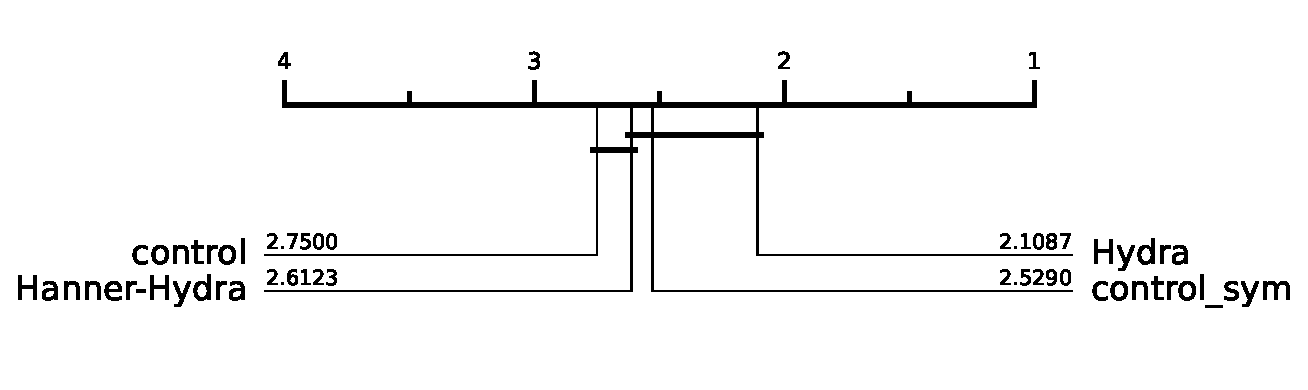
\includegraphics[width=0.8\linewidth]{figures/cd_all}
\caption{Critical-difference diagram over all 138 datasets: average ranks, with cliques
drawn by aeon's convention (one-sided Wilcoxon tests at a fixed level $\alpha/(k-1)$). The
pre-registered frequentist test is the Holm procedure of Table~\ref{tab:wilcoxon}; the
diagram can split pairs that the table does not.}
\label{fig:cd}
\end{figure}

The frequentist analysis agrees (Table~\ref{tab:wilcoxon}). No pair of arms differs
significantly at $\alpha=0.05$ after Holm's correction. A Friedman test over the four arms
is significant ($p=0.0002$), because Hydra ranks first more often: the average ranks are
2.11 for Hydra, 2.53 for \texttt{control\_sym}, 2.61 for \hh{} and 2.75 for
\texttt{control} (Figure~\ref{fig:cd}). On the subsets, two pairs reach significance:
\texttt{control\_sym} against Hydra on UEA ($-0.77$ points, Holm-adjusted $p=0.017$), and
\texttt{control\_sym} against \texttt{control} on UCR ($+0.09$ points, $p=0.045$), a
negligible effect of central symmetry.

\subsection{Comparison with published results}

\begin{table}[t]
\centering\small
% Generated by experiments/paper_tables.py; do not edit by hand.
\begin{tabular}{lrrlcl}
\toprule
Hanner-Hydra vs & Means (\%) & $\Delta$ & W/T/L & $P$(left / rope / right) & Label \\
\midrule
WEASEL 2.0 & 87.40 vs 87.38 & $+0.01$ & 58/3/51 & 0.441 / 0.080 / 0.479 & inconclusive \\
MiniRocket & 87.40 vs 87.44 & $-0.05$ & 57/4/51 & 0.474 / 0.110 / 0.416 & inconclusive \\
MultiRocket & 87.40 vs 88.14 & $-0.75$ & 42/5/65 & 0.991 / 0.003 / 0.007 & practically worse \\
HIVE-COTE 2.0 & 87.40 vs 89.14 & $-1.75$ & 30/4/78 & 1.000 / 0.000 / 0.000 & practically worse \\
\bottomrule
\end{tabular}

\caption{\hh{} against aeon's published 30-resample results on the 112 UCR datasets
(dataset means). Bayesian signed-rank test, ROPE $\pm0.5$; \emph{practically worse}:
$P(\Delta<-0.5)\ge0.95$.}
\label{tab:published}
\end{table}

Table~\ref{tab:published} compares \hh{} with the published results of four other methods
on the UCR datasets; aeon publishes these results for UCR only. \hh{} is on par with
WEASEL~2.0 and MiniRocket: the mean differences are below 0.05 points, but the posterior
is split between the two sides of the ROPE, so neither equivalence nor a difference is
shown. It is practically worse than MultiRocket ($-0.75$ points) and HIVE-COTE~2.0
($-1.75$). In two-sided Wilcoxon tests over all pairs of the eight methods (our four arms
and the four published ones), only HIVE-COTE~2.0 differs significantly from \hh{} ($p=2\times
10^{-6}$, $5\times10^{-5}$ after Holm's correction over 28 pairs). The published results use
different resample splits from ours, so this comparison is paired by dataset, not by
resample; our Hydra arm agrees with aeon's published Hydra results ($+0.33$ points,
posterior entirely in the ROPE).

\subsection{Ablations}

\begin{table}[t]
\centering\small
% Generated by experiments/paper_tables.py; do not edit by hand.
\begin{tabular}{lrrrlrr}
\toprule
Variant & Datasets & Mean (\%) & $\Delta$ vs default & W/T/L & $P$(rope) & $\Delta$ vs Hydra \\
\midrule
\texttt{center=False} & 138 & 83.69 & $-0.68$ & 26/8/104 & 0.995 & $-0.74$ \\
\texttt{center=True} & 138 & 84.35 & $-0.02$ & 60/8/70 & 1.000 & $-0.08$ \\
\texttt{features=hydra} & 138 & 84.37 & $+0.00$ & 0/138/0 & 1.000 & $-0.06$ \\
\texttt{max\_channels=32} & 7 & 65.78 & $-0.90$ & 2/0/5 & 0.285 & $-2.09$ \\
\texttt{max\_channels=auto} & 7 & 66.14 & $-0.53$ & 3/0/4 & 0.550 & $-1.72$ \\
\bottomrule
\end{tabular}

\caption{Exploratory ablations of \hh{}, 30 resamples each. $\Delta$ against the default
configuration (mixed centring, at most 8 channels, soft-max and hard-max counts) and
against Hydra; $P$(rope) from the Bayesian signed-rank test against the default. The
\texttt{max\_channels} variants differ from the default only on the 7 datasets with
$C\ge18$.}
\label{tab:ablations}
\end{table}

Table~\ref{tab:ablations} reports the pre-registered ablations, which are exploratory.
Without centring, accuracy drops by 0.68 points on average, mostly on UCR, and \hh{} loses
104 of the 138 datasets to the default. Most losses are small, though: the median is 0.24
points, 62\% of the datasets change by at most 0.5 points, and one dataset,
PigAirwayPressure, loses 27.9 points and alone moves the mean from $-0.49$ to $-0.68$. The
signed-rank test is robust to such an outlier, so its posterior lies in the ROPE
($P=0.995$). Centring every group instead of every second one is
equivalent to the default. Hard-min counts in place of the hard-max counts give the same
accuracy on all 4,140 dataset resamples, and all 4,140 prediction files are
byte-identical to those of the default. This confirms the permutation argument of Proposition~\ref{prop:hardmin}
in the implementation, which takes the minimiser as the antipode of the maximiser; it is not
a test of Hydra's first-minimiser rule. Larger channel subsets do not help on the 7 high-channel datasets ($-0.90$ and $-0.53$
points; W/T/L 2/0/5 and 3/0/4, $P(\text{rope})=0.285$ and $0.550$, so inconclusive), which
makes a lack of channel coverage an unlikely explanation for the UEA gap.

\section{Related work}
\label{sec:related}

\paragraph{Random convolutional kernels.} ROCKET classifies time series with a linear
model on features pooled from thousands of random convolutional kernels
\citep{dempster2020rocket}. MiniRocket replaces the random kernels by a small fixed set with
two weight values \citep{dempster2021minirocket}, MultiRocket adds pooling operators and the
first difference \citep{tan2022multirocket}, and Hydra organises random kernels into
competing groups \citep{dempster2023hydra}. QUANT, an interval method, classifies quantiles
over fixed intervals with extremely randomised trees, in less than 15 minutes of
single-core compute for 142 UCR datasets \citep{dempster2024quant}. In the
most recent bake-off, the concatenation of MultiRocket and Hydra features and the HIVE-COTE
2.0 ensemble were the most accurate methods on the UCR archive
\citep{middlehurst2024bakeoff,middlehurst2021hc2}. Two lines of work reduce the cost of
these transforms after the fact: pruning kernels or features, which can remove most of them
with little loss of accuracy \citep{salehinejad2022srocket,uribarri2024detach}, and
combining fast transforms with stronger models, such as stacked ensembles of Hydra and
QUANT \citep{maniar2025metalearning} or tabular in-context learners on ROCKET features
\citep{orourke2026rocketpfn}. \hh{} takes a different route: it changes what a group is, so
that the cost of finding a group's winner no longer grows with its size. Its features could
enter the same combinations.

\paragraph{Low-precision and edge variants.} The closest work is NanoHydra
\citep{cioflan2025nanohydra}, which runs Hydra on a microcontroller with binary kernels
($\pm1$), integer arithmetic and a quantised linear classifier. Its groups remain random
sets of kernels that are evaluated one by one. In its own evaluation on the UCR archive,
NanoHydra averages 83.81\% against 85.31\% for Hydra (Hydra's number as reported by
\citet{schaefer2023weasel2}), although its numbers are the best of several runs per
dataset. The two approaches address different costs: NanoHydra makes each kernel cheaper,
and \hh{} makes the whole group cheaper. A Hanner cube group contains all $2^\ell$ sign
vectors on its taps and finds the winner in $O(\ell)$ operations; a group of $k$ random
sign vectors needs $k$ dot products. Combining Hanner groups with NanoHydra's integer
pipeline is a natural next step. More broadly, ternary and binary networks
\citep{li2016ternary,rastegari2016xnor} and adder networks \citep{chen2020addernet} reduce
the cost of each learned weight; we do not learn weights and instead remove the dependence
on the number of kernels in a group.

\paragraph{Dictionary and pattern-based methods.} Dictionary methods classify series by
counting symbolic words, from SAX \citep{lin2007sax} to WEASEL~2.0
\citep{schaefer2023weasel2}, which is about as accurate as MiniRocket. Hanner features are
counts of words too: sign patterns on subsets of taps, weighted by the response. Sign
patterns of neighbouring samples are also the basis of one-dimensional local binary
patterns \citep{kaya2014lbp}. Ordinal patterns \citep{bandt2002permutation} are related but
different: they record the rank order of the samples in a window, not their signs.

\paragraph{Hashing and max-affine units.} The winner of a cube group is a sign pattern, the
code of hyperplane hashing \citep{charikar2002simhash}, and the winner of a cross-polytope
group is a signed coordinate, the code of cross-polytope hashing
\citep{andoni2015crosspolytope}; Section~\ref{sec:interpretation} makes this precise.
Winner-take-all hashing records the index of the largest of several coordinates
\citep{yagnik2011wta}, which is what Hydra's counts record for kernel responses. A group's
largest response, the support function of a polytope, is also the output of a maxout unit;
maxout polytopes \citep{balakin2025maxout} study the polytopes that networks of such units
define. We found no work that chooses competing kernels for the structure of their
polytope, or that finds a group's winner faster than by evaluating each kernel.

\paragraph{Evaluation.} We follow the bake-off protocol of 30 stratified resamples
\citep{ruiz2021multivariate,middlehurst2024bakeoff} on the UCR and UEA archives
\citep{dau2019ucr,bagnall2018uea}, with aeon's implementations and published results
\citep{middlehurst2024aeon}. Our primary test is the Bayesian signed-rank test of
\citet{benavoli2017bayesian}, which turns a margin of practical equivalence into a decision
rule, with Wilcoxon--Holm tests and critical-difference diagrams
\citep{demsar2006statistical} as secondary analyses; pairwise comparisons also avoid the
dependence of critical-difference diagrams on the set of compared methods
\citep{ismailfawaz2023mcm}. The UCR and UEA datasets are small, which favours
low-variance methods; the MONSTER collection \citep{dempster2025monster} offers large
datasets on which the speed of \hh{} would matter more.

\section{Discussion and limitations}
\label{sec:discussion}

\paragraph{What the result shows.} On the pre-registered benchmark, the structure of a
Hanner group buys speed and memory at a cost in accuracy that stays within the margin of
$\pm0.5$ points over all 138 datasets: \hh{} is practically equivalent to Hydra and
$11.2\times$ faster. It
does not buy accuracy. \hh{} is practically equivalent to both matched controls on every
subset and every metric, so the tree adds no measurable accuracy over random ternary
groups of the same size and sparsity; its contribution is the cost of finding the winner. Nor is \hh{} a more accurate classifier than the state of the art: MultiRocket and
HIVE-COTE~2.0 are practically better on the UCR datasets (Table~\ref{tab:published}).

\paragraph{The UEA gap.} On the 26 UEA datasets, \hh{} is 0.54 points behind Hydra and
\emph{not worse} is not shown. The gap is concentrated on the 7 datasets with at least 18
channels ($-1.19$ points; PEMS-SF $-3.08$) and smaller on the other 19 ($-0.30$, including
the largest single loss, AtrialFibrillation with $-4.89$ on 15 test cases). The symmetric
control has the same gap on the same 7 datasets ($-1.15$), so the gap comes with ternary
groups of this kind, not with the tree. Larger channel subsets do not close it (the ablation
is inconclusive on 7 datasets), and in an exploratory diagnosis on development datasets
before the freeze, Hydra stayed ahead when it saw the same number of channel draws as
\hh{}. Both point to the groups or their features rather than to channel coverage, but
neither settles the question. Balanced accuracy and macro-F1 show a slightly larger gap to
Hydra than accuracy, which suggests somewhat larger losses on minority classes; against
Hydra, both are inconclusive.

\paragraph{Limitations.}
\begin{itemize}
\item \emph{Equivalence, not superiority}, under a margin of $\pm0.5$ points on dataset
  means; smaller differences are not resolved.
\item \emph{One machine.} All times come from one CPU (Apple M4) with one thread. The ratios
  may differ on other processors, with several threads, or on accelerators. Cache-miss
  rates could not be measured and were dropped, as the pre-registration allowed.
\item \emph{What the timings include.} Hydra's timed region includes aeon's conversion to
  and from PyTorch tensors, as aeon runs it; we did not measure that conversion's share of
  the $11.2\times$. The controls were timed with dense ternary dot products, so the
  $3.8\times$ attributed to the tree is an upper bound on its gain over the best ternary
  implementation. The timed kernels use floating point; the multiplication-free form of
  Section~\ref{sec:operations} was not timed.
\item \emph{Datasets.} Only equal-length series were used, so 4 UEA datasets are excluded,
  and the UCR and UEA datasets are small \citep{dempster2025monster}. The published
  comparators use different resample splits from ours and are paired by dataset only.
\item \emph{The protocol} was pre-registered as a tagged document in our own repository,
  not in a public registry.
\item \emph{The theory.} The extremal properties of Hanner polytopes motivated the choice
  of the family, but the method does not use them, and the most general one rests on an
  unrefereed manuscript (Section~\ref{sec:hanner}).
\end{itemize}

\paragraph{Future work.} The natural next step is an integer implementation on a
microcontroller, compared with NanoHydra \citep{cioflan2025nanohydra} on the same hardware;
the multiplication-free form of the group evaluation makes this direct. A sparse ternary
control kernel would measure the tree's gain over the best ternary implementation, of
which the $3.8\times$ is an upper bound. Hydra is most
accurate in combination with MultiRocket features \citep{middlehurst2024bakeoff}, and
\hh{} features can enter the same combinations, or those with QUANT and tabular models
\citep{maniar2025metalearning,orourke2026rocketpfn}. Large datasets
\citep{dempster2025monster}, where the speed and memory savings matter most, series of
unequal length, and data-dependent rather than random trees are further directions.

\section{Reproducibility}
\label{sec:reproducibility}

Everything needed to check or extend the results is public.

\paragraph{Code.} The \texttt{hanner-hydra} repository
(\url{https://github.com/jorgebmann/hanner-hydra}, BSD-3-Clause) contains the NumPy
reference implementation, the Numba kernels with tests that they reproduce the reference bit
for bit, the aeon-compatible estimators, and every experiment and analysis script. The
dependency versions are pinned (aeon 1.6.0, NumPy 2.3.5, scikit-learn 1.9.1, Numba 0.63.1,
PyTorch 2.15.0).
\todo{Zenodo DOI of the code release.}

\paragraph{Pre-registration.} The protocol of Section~\ref{sec:protocol} is the document
\texttt{docs/preregistration.md}, together with the code of the harnesses. Its public
edition differs from the frozen document only in wording (references to internal
planning documents) and in a section listing the one deviation after the freeze.

\paragraph{Results.} The release \texttt{results-v1} (CC BY 4.0), archived on Zenodo
\citep{bahlmann2026results}, holds the per-resample
results of all arms and ablations, all per-case test predictions, the timing passes, the
memory measurements and the secondary analyses, with a SHA-256 manifest. Extracted in a
checkout of the repository, it lets the analysis scripts reproduce the results without
rerunning the experiments, and \texttt{experiments/paper\_tables.py} regenerates every
table of this paper from it. Third-party results (aeon's published results and the Hydra
paper's) are not redistributed; the scripts download them, and the release records their
checksums.


\section*{Competing interests}
The author intends to offer commercial products and services based on the method described
here. No patent has been filed or is planned; the reference implementation is open source
(BSD-3-Clause) and the results are released under CC BY 4.0.

\section*{Funding}
This work received no specific funding.

\bibliographystyle{plainnat}
\bibliography{references}

\end{document}
